\documentclass[11pt, fleqn]{article}
\usepackage[margin=2cm, a4paper]{geometry} 
\usepackage[colorlinks=true, linkcolor=black]{hyperref}
\usepackage{parskip} % Paragraphs are separated by a blank line w/o indenting
\usepackage{graphicx}
\usepackage{float}
\usepackage{grffile}
\usepackage{subcaption}
\usepackage{csvsimple}
\usepackage{booktabs}
\usepackage[T1]{fontenc} % recognize the underscore char
\usepackage{array}
\usepackage{fancyvrb}
\usepackage{float}
\usepackage{xcolor}
\usepackage{amsmath}
\floatstyle{plaintop}
\restylefloat{table}

\title{A tutorial on quadratic programming \\
\medskip
\large An example of deconvolution of a mixed population of cells}

\author{Dario Beraldi \\
\href{https://github.com/dariober/quadratic-programming-deconvolution}{https://github.com/dariober/quadratic-programming-deconvolution}}
\date{\today}

\begin{document}
\renewcommand{\abstractname}{\vspace{-\baselineskip}}

\maketitle
\tableofcontents
\pagebreak

\begin{abstract}
\noindent
This tutorial shows how to use quadratic programming, as implemented in the R
packages \texttt{pracma} and \texttt{quadprog}, to solve the problem of
deconvolving a mixed cell population into individual subpopulations.

\noindent
Quadratic programming solves the problem of optimizing (minimizing or
maximizing) a quadratic function of several variables subject to linear
constraints on these variables.  Among many other applications, it can be
used to deconvolve a mixed population of cells into individual
subpopulations given, for example, the expression profile of the mixed
population and the reference profiles of the single subpopulations

\noindent
Quadratic programming has been implemented in various languages including R and
python. However, I found the documentation and examples quite abstract and difficult to 
apply to real problems.

\noindent
I wrote this document for my own reference and hopefully to be useful to
others, but it is not meant to be authoritative in any way. Feel free to open
an issue to send any comment, question, or correction. 
\end{abstract}

\section{The problem}

This fictitious example comes from biology but it should be understandable to
anyone. 

Imagine you have a sample of cells composed by a mixture of
life stages, say young, adult, old, male gametes and female gametes, and we want to estimate the
percentage of each stage. For this mixed population we have the level of
expression of 1000 genes (for example from bulk RNA-Seq or microarray). From literature we
have the reference expression of these genes of the pure life stages. So the data at hand looks like:

\begin{Verbatim}[formatcom=\color{violet}, fontsize=\small]
# Reference gene expression of pure life stages:
          Y     A     O     F     M
  gene_1  0.588 1.85  5.64  4.94  6.67
  gene_2  3.579 5.08  9.82  7.02 14.01
  gene_3  2.545 5.86 10.01 10.31  8.48
  gene_4  1.290 5.04 11.17 15.32  8.22
  gene_5  4.132 2.12 13.21 13.24  9.67
  ---                                    
gene_996  3.045 8.20  9.45  5.00 10.01
gene_997  4.885 2.51  9.13 11.12 13.69
gene_998  3.730 7.78 11.56  8.91  9.68
gene_999  2.385 6.23  5.81 10.51 10.90
gene_1000 1.364 5.64  4.76  8.40 10.41

# Gene expression of our mixed population:
   gene_1  4.74
   gene_2  9.37
   gene_3 11.88
   gene_4 12.62
   gene_5 13.93
   ---          
 gene_996 10.11
 gene_997 11.13
 gene_998 12.33
 gene_999  8.80
gene_1000  5.63
\end{Verbatim}

How can we deconvolute the mixed population into the proportions of individual stages?

\section{Quadratic programming}

The expression of each gene $y_{i}$ in the mixed population comes from the same (linear) combination of 5 individual stages $\beta$. So the problem is to solve the system of equations:

$y_{1} = \beta_{Y} x_{1} + \beta_{A} x_{1} + \beta_{O} x_{1} + \beta_{M} x_{1} + \beta_{F} x_{1}$

$y_{2} = \beta_{Y} x_{2} + \beta_{A} x_{2} + \beta_{O} x_{2} + \beta_{M} x_{2} + \beta_{F} x_{2}$

$y_{3} = \beta_{Y} x_{3} + \beta_{A} x_{3} + \beta_{O} x_{3} + \beta_{M} x_{3} + \beta_{F} x_{3}$

\dots

$y_{1000} = \beta_{Y} x_{1000} + \beta_{A} x_{1000} + \beta_{O} x_{1000} + \beta_{M} x_{1000} + \beta_{F} x_{1000}$

So we need find the combination of $\beta_{Y}, ..., \beta_{F}$ to solve the
system. Because the system is overdetermined and because of measurement errors,
we cannot find a single, perfect solution. Most important, \textbf{we need to
constraint the coefficients} $\beta$ to be: 1) $\geq 0$ and 2) $\sum_{i=1}^{n}
\beta_{i} = 1$ (proportions must sum to 1).

This is an optimization problem the can be solved via 
\href{https://en.wikipedia.org/wiki/Quadratic_programming}{quadratic
programming}, find a the vector of coefficients $\mathbf{x}$ that minimizes

\begin{equation}
\frac{1}{2} \mathbf{x}^\mathrm{T} Q\mathbf{x} + \mathbf{c}^\mathrm{T} \mathbf{x}
\end{equation}

subject to

$\mathbf{Ax} \preceq \mathbf{b}$ (each entry in $\mathbf{Ax}$ is less then or equal the corresponding entry in $\mathbf{b}$)

If our reference expression matrix is $\mathbf{X}$ and the vector of gene
expressions from the mixed population is $\mathbf{y}$, $\mathbf{Q} =
\mathbf{X}^\mathrm{T}\mathbf{X}$ and $\mathbf{c} =
\mathbf{X}^\mathrm{T}\mathbf{y}$. Matrix $\mathbf{A}$ and vector $\mathbf{x}$
specify the constraints (see below).

\section{Set up}

In this section we install the required packages and generate a toy dataset to demostrate the deconvolution

\begin{Verbatim}[formatcom=\color{violet}, fontsize=\small]
install.packages('pracma')     # Also installs quadprog
install.packages('data.table') # Not strictly needed
install.packages('ggplot2')    #

library(pracma)
library(data.table)
library(ggplot2)
\end{Verbatim}

Prepare test data

\begin{Verbatim}[formatcom=\color{violet}, fontsize=\small]
set.seed(1234)

n <- 1000
base <- rnorm(n= n, mean= 0, sd= 1)
dat<- data.table(value= c(
    base + rnorm(n= n, mean= 3, sd= 1),
    base + rnorm(n= n, mean= 5, sd= 2),
    base + rnorm(n= n, mean= 8, sd= 3),
    base + rnorm(n= n, mean= 10, sd= 4),
    base + rnorm(n= n, mean= 12, sd= 5)
    ),
    stage= rep(c('Y', 'A', 'O', 'F', 'M'), each= n),
    gene= paste('gene', rep(1:n, times= 5))
)
dat[, stage := factor(stage, levels= c('Y', 'A', 'O', 'F', 'M'))]

ref <- dcast.data.table(data= dat, gene ~ stage, value.var= 'value')
gene <- ref$gene
ref[, gene := NULL]
ref <- as.matrix(ref)
rownames(ref) <- gene
\end{Verbatim}

We create a vector of gene expression values by mixing the 5 stages in the
matrix \texttt{ref}. For the sake of example, we create an unphysical mixture
where one stages has negative percentage and the sum of proportions is different
from 1 (in real experiments this could happen from random and non-random
variation). In this way we show that optimization under constraints still
returns meaningful estimates.

\begin{Verbatim}[formatcom=\color{violet}, fontsize=\small]
set.seed(1234)
mix <- ref %*% c(-0.1, 0.2, 0.5, 0.3, 0.2) + rnorm(n= nrow(ref), sd= 1)

gg<- ggplot(data=  rbind(dat[, list(value, stage)], 
        data.table(value= mix[,1], stage= 'Mix')),aes(x= value, fill= stage)) +
    geom_histogram(bins= 30, alpha= 0.5, position= 'identity', colour= 'white')
ggsave('figures/reference_samples.pdf', width= 14, height= 10, units= 'cm')
\end{Verbatim}

\begin{figure}[H]
    \center
    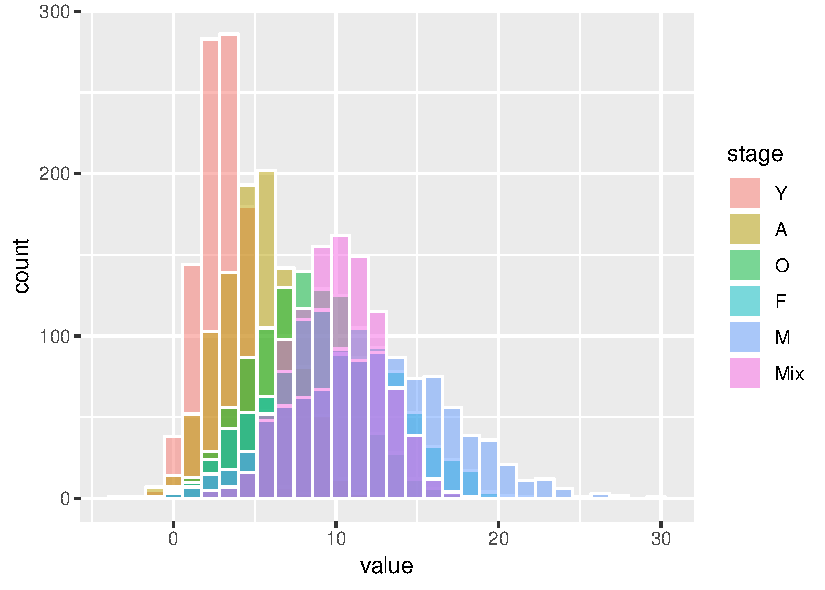
\includegraphics[height=0.5\textwidth]{figures/reference_samples.pdf}
    \caption{Distribution of gene expression values for the reference samples
    and the mixed sample}
    \label{fig:reference_samples}
\end{figure}

\section{Deconvolution}

\subsection{Unconstrained optimization}

Without constraints the quadratic programming solution is equivalent to the
ordinary least square used in linear regression. This approach gives the best
solution in terms of minimizing the discrepancy between observed and fitted
values but it can give negative coefficients and the sum of coefficients may
not equal 1. In other words, the best mathematical solution is not physically
possible.

\begin{Verbatim}[formatcom=\color{violet}, fontsize=\small]
x <- lsqlincon(ref, mix)
x
#     [,1]
# Y -0.097  # -ve proportion!
# A  0.198
# O  0.496
# F  0.306
# M  0.196

sum(x)
# [1] 1.099684

lmx <- lm(mix ~ 0 + ref) # Linear regression
lmx$coefficients
#  refY   refA   refO   refF   refM 
#-0.097  0.198  0.496  0.306  0.196 

\end{Verbatim}

\subsection{Vanilla constraints}

For deconvolving a mixture of stages into meanigful individual stages we require:

\begin{itemize}
    \item The percentage of a stage cannot be negative as this would be
        unphysical. \emph{I.e.}, $\mathbf{x} \succeq 0$, each element of the
        solution vector is greater than or equal to zero.
    \item The percentages of each stage in the mixture sums up to 100\%.
        \emph{I.e.}, $\sum_{i=1}^{n} x_{i} = 1$, only the reference stages make
        up the mixture. Maybe in other cases we want the sum to be less than 1
        or $a \leq x \leq b$ if we know for sure that the mixure contains
        something other than the reference stages? See below for more complex constraints.
\end{itemize}

Using the function \texttt{lsqlincon} in the \texttt{pracma} package, we set
the lower and upper boundaries of the coefficients in $\mathbf{x}$ to be $[0,
1]$. (The upper boundary set to 1 is redundant here since the sum must be $\leq
1$ anyway):

\begin{Verbatim}[formatcom=\color{violet}, fontsize=\small]
lb <- rep(0, ncol(ref))
ub <- rep(1, ncol(ref))
\end{Verbatim}

Now we set the matrix and vector of equality constraints to require the sum of
coefficients to be 1. Since we have only one equality constraint the matrix and
vector will have one row and one element, respectively.

\begin{Verbatim}[formatcom=\color{violet}, fontsize=\small]
Aeq <- matrix(rep(1, ncol(ref)), nrow= 1)
Aeq
#      [,1] [,2] [,3] [,4] [,5]
# [1,]    1    1    1    1    1

beq <- c(1)
\end{Verbatim}

And solve. \texttt{x} is the composition of stages in the observed mixture \texttt{mix}:

\begin{Verbatim}[formatcom=\color{violet}, fontsize=\small]
x <- lsqlincon(ref, mix, Aeq= Aeq, beq= beq, lb= lb, ub= ub)
x
# [1] 0.000 0.000 0.427 0.323 0.250
\end{Verbatim}

Check the $\sum_{i=1}^{n} x_{i} = 1$ and $\mathbf{Ax} = \mathbf{b}$:

\begin{Verbatim}[formatcom=\color{violet}, fontsize=\small]
sum(x) # 1
Aeq %*% x == beq # TRUE
\end{Verbatim}

So our mixed sample contains 0\% of stages Young and Adult, and 42.7\% of Old,
32.3\% Female gametocytes and 25.0\% Male gametocytes.

\subsection{Additional constraints}

Additional equality and inequality constraints can be set by adding rows to the
matrices \texttt{Aeq} and \texttt{A} and to the corresponding vectors
\texttt{beq} and \texttt{b}.  Let's add additional constraints for the sake of
example. 

\begin{itemize}
    \item The sum of the first two coefficients must be equal to 0.2. This is an
        additional equality constraint
    \item The sum of the forth and fifth coefficient must be less then or equal to 0.5. This is an inequality constraint.
    \item The sum of first and third constraint must be greater then or equal to 0.4. Note the negative sign in $\mathbf{A}$ and $\mathbf{b}$ to specify $\geq 0.4$. 
        This is because \texttt{lsqlincon} is setup to use $\mathbf{Ax} \preceq \mathbf{b}$
\end{itemize}

\begin{Verbatim}[formatcom=\color{violet}, fontsize=\small]
Aeq <- matrix(c(rep(1, ncol(ref)), 
        1, 1, 0, 0, 0), nrow= 2, byrow= TRUE)
Aeq
#     [,1] [,2] [,3] [,4] [,5]
#[1,]    1    1    1    1    1
#[2,]    1    1    0    0    0

beq <- c(1, 0.2)

# Inequality constraint(s)
A <- matrix(c(0,  0,  0, 1, 1,
              -1, 0, -1, 0, 0), nrow= 2, byrow= TRUE) 
A
#[,1] [,2] [,3] [,4] [,5]
#[1,]    0    0    0    1    1
#[2,]   -1    0   -1    0    0

b <- c(0.5, -0.4)

x <- lsqlincon(ref, mix, Aeq= Aeq, beq= beq, A= A, b= b, lb= lb, ub= ub)
x
# 0.044 0.156 0.356 0.189 0.255
\end{Verbatim}

As before, check the constraints are satisfied:

\begin{Verbatim}[formatcom=\color{violet}, fontsize=\small]
# Check Aeq * x = beq:
Aeq %*% x
#     [,1]
#[1,]  1.0
#[2,]  0.2

# Check A * x <= b
A %*% x
#           [,1]
#[1,]  0.4438455
#[2,] -0.4000000

\end{Verbatim}


\subsection{Deconvolution using \texttt{quadprog}}

The workhorse of \texttt{lsqlincon} is \texttt{solve.QP} from the
\texttt{quadprog} package (installed together with \texttt{pracma}).
\texttt{lsqlincon} has an easy interface to input data and constraints while
\texttt{solve.QP} is more difficult to understands but its interface
is closer to the mathematical definition of the quadratic programming problem.
Some python implementations of quadratic programming seems to be similar to
\texttt{solve.QP} in terms of interface. Here's how to use \texttt{solve.QP}
directly:

\begin{itemize}
    \item Argument \texttt{Dmat} is $\mathbf{X}^\mathrm{T}\mathbf{X}$ where
        $\mathbf{X}$ is the matrix of reference stages \texttt{ref}
    \item \texttt{dvec} is the vector $\mathbf{c}$ in the quadratic programming
        equation. It is obtained from $\mathbf{X}^\mathrm{T}\mathbf{y}$ where
        $\mathbf{y}$ is the vector to be deconvoluted (\texttt{mix}).  
    \item \texttt{Amat}, \texttt{bvec}: \texttt{Amat} is the matrix of equality
        and inequality constraints. In contrasts to \texttt{lsqlincon}, all the
        constraints are specified here and in the corresponding vector
        \texttt{bvec}. This means that also the lower and upper bounds of the
        coefficients ($[0, 1]$) must be input in \texttt{Amat} and \texttt{bvec}. 
    \item \texttt{meq} tells \texttt{solve.QP} that the first
        \texttt{meq} rows of \texttt{Amet} and \texttt{bvec} are equality
        constraints, the other rows are inequalities.
\end{itemize}

Let's translate \texttt{lsqlincon} to \texttt{solve.QP}. We use the constraint
matrices and vectors from above but we flip the signs since \texttt{solve.QP}
is setup to use $\mathbf{Ax} \succeq \mathbf{b}$. The lower and upper bounds of
the coeffcients, arguments \texttt{lb} and \texttt{up} in \texttt{lsqlincon},
are also inequality constraints so we translate them as additional rows to
\texttt{Amat} and \texttt{bvec}.

\begin{Verbatim}[formatcom=\color{violet}, fontsize=\small]
library(quadprog)

Dmat <- t(ref) %*% ref
dvec <- t(ref) %*% mix

# Equality and inequality matrix and corresponding vector
Amat <- rbind(-Aeq, -A, diag(ncol(ref)), -diag(ncol(ref)))
bvec <- c(-beq, -b, rep(0, ncol(ref)), rep(-1, ncol(ref))) 

meq <- nrow(Aeq) # The first N rows in Amat are equality constraints
\end{Verbatim}

Here's a review of the (in)equality matrix and vector $\mathbf{A b}$

\begin{Verbatim}[formatcom=\color{violet}, fontsize=\small]
       Amat             bvec
 [1]   -1 -1 -1 -1 -1   -1.0    # Equality constraints
 [2]   -1 -1  0  0  0   -0.2    # 
 [3]    0  0  0 -1 -1   -0.5    |
 [4]    1  0  1  0  0    0.4    |
 [5]    1  0  0  0  0    0.0    |
 [6]    0  1  0  0  0    0.0    |
 [7]    0  0  1  0  0    0.0    |
 [8]    0  0  0  1  0    0.0    | Inequality constraints
 [9]    0  0  0  0  1    0.0    |
[10]   -1  0  0  0  0   -1.0    |
[11]    0 -1  0  0  0   -1.0    |
[12]    0  0 -1  0  0   -1.0    |
[13]    0  0  0 -1  0   -1.0    |
[14]    0  0  0  0 -1   -1.0    |
\end{Verbatim}

\begin{itemize}
    \item Row 1: The sum of coefficients must be 1. All negative because quadprog wants $\mathbf{Ax} \succeq \mathbf{b}$ 
    \item Row 2: Sum of first and second coefficient must be 0.2
    \item Row 3: Sum of forth and fifth coefficient must be $\leq 0.5$
    \item Row 4: Sum of first and third coefficient must be $\geq 0.4$ (Note positive sign)
    \item Rows 5-9: Each coefficient must be $\geq 0$
    \item Rows 10-14: Each coefficient must be $\leq 1$ (redundant because of row 1)
\end{itemize}

Now we can solve the system. Note that \texttt{Amat} is transposed. The output of
\texttt{solve.QP} contains the solution and additional information. The
solution is the same as with \texttt{lsqlincon} and the unconstrained solution
is the same as with ordinary least square.

\begin{Verbatim}[formatcom=\color{violet}, fontsize=\small]
solve.QP(Dmat= Dmat, dvec= dvec, Amat= t(Amat), bvec= bvec, meq= meq)
# $solution
# [1] 0.04384555 0.15615445 0.35615445 0.18876468 0.25508087
#
# $unconstrained.solution
# [1] -0.09676762  0.19822490  0.49608145  0.30645299  0.19569261
\end{Verbatim}

\section{Assessing the quality of the estimates}

\begin{itemize}
    \item Get fitted values and residuals
    \item Calculate deviance, RMSE, MAE
    \item Test for contribution of a stage to be different from 0
\end{itemize}

Fitted values

\begin{equation}
    \mathbf{\hat y} = \mathbf{X} \mathbf{x}
\end{equation}

\begin{equation}
RMSE = \sqrt{\frac{\sum_{i=1}^N (\hat y_i - y_i)^2}{N}}
\end{equation}

\begin{equation}
MAE = \frac{\sum_{i=1}^N\left| \hat y_i - y_i\right|}{N}
\end{equation}

\begin{Verbatim}[formatcom=\color{violet}, fontsize=\small]
fitted.values <- ref %*% x
residual.values <- mix - fitted.values
rmse <- 


rssq <- sum(residual.values^2)

fitted.values <- ref[, 2:5] %*% x2
residual.values <- mix - fitted.values
rssq2 <- sum(residual.values^2)
1 - pchisq(rssq - rssq2, 1)
\end{Verbatim}

\section{References and credits}

\begin{itemize}
    \item Francisco Avila Cobos, Jo Vandesompele, Pieter Mestdagh, Katleen De
        Preter, \href{https://doi.org/10.1093/bioinformatics/bty019}{Computational deconvolution of transcriptomics data from mixed
        cell populations}, Bioinformatics, Volume 34, Issue 11, 01 June 2018,
        Pages 1969-1979

    \item https://stats.stackexchange.com
        \href{https://stats.stackexchange.com/questions/21565/how-do-i-fit-a-constrained-regression-in-r-so-that-coefficients-total-1}{How
        do I fit a constrained regression in R so that coefficients total = 1?}

    \item R package \href{https://CRAN.R-project.org/package=pracma}{pracma} 
        
    \item R package \href{https://CRAN.R-project.org/package=quadprog}{quadprog}

    \item The matlab documentation for \href{https://uk.mathworks.com/help/optim/ug/lsqlin.html}{lsqlin}

\end{itemize}

\end{document}
